\chapter{The Bracelet}

The interactive bracelet consists mainly of an electronic ink display and several touch sensors for conscious interaction and a motion sensor for gesture recognition. The bracelet's design focuses on wearing comfort, low weight and small error of unintended activation.

\section{Manufacturing Techniques}

In this section, the various methods and tools used for designing and manufacturing the bracelet prototypes will be explained in detail.

\subsection{Computer Aided Design}
%TODO: references
% http://www3.ul.ie/~rynnet/parametricmodellingbasics-solidworks.php
%TODO pictures
In the beginning of a design iteration, a virtual model of the desired object is built with a 3D \ac{CAD} program. For all designs in the context of this thesis, the open source \ac{CAD} modeler FreeCAD\cite{freecad} was used. This program classifies itself as a general purpose 3D parametric modeler. A typical work-flow when designing a bracelet is as follows:

The model's basis is a circumference sketch for the bracelet. As the human wrist does not follow a circular shape, all designs made for this thesis are based on an oval circumference. In FreeCAD, this is realized by a composition of arcs and straight lines. It is important to constraint the sketch with radii, lengths and angles as well as symmetries or perpendicular constraints. The sketch should be fully constrained (i.e. leaving no degrees of freedom) before moving on to the next step, also with respect to the printing of the finished design.

In the next step one or more profile cuts are added to the circumference. They define the thickness and shape of the bracelet at different points along the oval circumference. For increased comfort, the bracelet should be as slim as possible, especially on the "backside" below the palm. In more complicated designs, an alternative to complex sketches for the profiles is the creation of multiple, overlaid sketches as a preparation for a subtraction operation in the later process. All those profiles need to be fully constrained as well.

After the circumference as well as one or more profiles are added to the design, a first solid is created by sweeping the profile(s) around the circumference curve. This operation creates a basic shape that can be refined further on, typically by chamfering or filleting the edges with respect to increased wearing comfort. If a complex shape is desired, multiple sweeps can be generated and used in boolean operations such as union or subtraction. This is the usual approach for most bracelet designs.

The last step in the design process is usually the finishing of the \ac{CAD} model. In the bracelet case, this translates to edge smoothing with chamfer or fillet tools. Smoothed edges increase the overall wearing comfort of a bracelet, so they are very desired on edges that contact with the skin.

The finished designs are then exported as mesh files (usually in \ac{STL} format) for printing.

\subsection{3D Printing}
%TODO a little more about the powder technique, maybe historical background? -> Wikipedia
%TODO Mechanisms and Mechanical Devices Sourcebook, TIB
% http://www.sciencedirect.com/science/book/9780121742317
% http://www.google.com/patents/US5340656
% http://en.wikipedia.org/wiki/Z_Corporation
% http://www.3dsystems.com/about-us
The \ac{HCI} group's workshop includes a powder bed and inkjet head 3D printer, a ProJet 360 by 3DSystems, Inc\cite{printer}. This manufacturing technique was developed in 1989 by the \ac{MIT} \cite{sachs1994three} and then licensed to the Z Corporation in 1995. On January 3, 2012, Z Corporation was acquired by 3DSystems, Inc.

When printing an object, the print bed is filled first with a base layer of powder. The powder used by the printer is called VisiJet PXL, a plaster-like substance. After filling the bed, a standard inkjet printhead is cleaned and prepared for the printing process. Immediately after this setup is complete, the additive manufacturing process starts.

The model is created by printing the binder fluid onto the plaster. After each printed layer, a new thin layer of powder is added to the print bed. The ProJet360 allows for a layer thickness of 0.1 mm with a vertical build speed of 2 cm per hour\cite{datasheet_printer}. This allows even delicate structures without any additional supports, since the printed object is surrounded and therefore supported by plaster powder during the production process. The only drawback of this printing process is that it doesn't support closed, hollow objects since there is no possibility of removing the enclosed excess powder after the process has finished. When designing models for 3D printing, this constraint has to be kept in mind.

The finished object is then carefully removed from the build bed and any excess powder is gently brushed or blown off. The printer offers a cleaning chamber with a pressurized air pistol and a vacuuming system to assist in that task. Without further hardening, the objects are very fragile and easy to break, even with the pressurized air pistol included in the printer. In order to drastically increase the strength of the prints, they are infiltrated with a fluid after they were thoroughly cleaned. Prints produced by the ProJet 360 can be infiltrated with one of three different substances with varying characteristics: The ColorBond "instant-cure infiltrant", the two-part StrengthMax infiltrant "ideal for functional models", and the Salt Water Cure "eco-friendly and hazard-free infiltrant"\cite{datasheet_printer}. All prints produced for this thesis were infiltrated with ColorBond.

The infiltration step adds strength and hardens the material, resulting in a sturdy printed object. However, the objects created with this technique are very rigid and any bending load might break them easily. Wall strengths of 1.5 mm and up have been proven sturdy enough for a bracelet shape, although this also depends on the object geometry.

\subsection{Silicone Casting}
%TODO mold making
%TODO are those the right silicone names?
% http://www.npl.co.uk/science-technology/mass-and-force/hardness/rubber-hardness
% https://www.google.com/patents/US1770045
% http://www.calce.umd.edu/TSFA/Hardness_ad_.htm#3.5
% ISO 7619 for scale OO?
Another manufacturing process for bracelet prototypes used in this thesis is liquid silicone casting. Two different types of silicone were used for making various bracelet prototypes, both from manufacturer Smooth-On: Sorta-Clear 37 and Mold Star 15 Slow.

The most important characteristic for silicone in prototype production is the hardness, measured in Shore (after Albert F. Shore) or Durometer. It measures the indentation of a material with a special device which is also called Shore Durometer. It consists of a hardened steel rod with a finer tip and is available in two versions, since there are two different scales for Shore hardness (cf. table \ref{tab:shore}). The Shore A scale is designed for softer materials and the Shore D scale for harder ones, but they do overlap, so a material classified in Shore D hardness is not necessarily harder than another material classified in Shore A hardness. Each scale ranges from values 0 to 100, higher numbers indicate higher material resistance. The Shore hardness is specified in EN ISO 868.

\begin{table}
	\myfloatalign
	\begin{tabularx}{\textwidth}{clcc} \toprule
		\tableheadline{Type} & \tableheadline{Configuration} & \tableheadline{Diameter} & \tableheadline{Spring Force}\\ 
		\midrule
		A & $35\degree$ & $1.4$ mm & $8.06$ N \\
		D & $30\degree$ & $1.4$ mm & $44.46$ N\\
		OO & $1.2$ mm in spherical radius & $2.4$ mm & $1.11$ N \\
		\bottomrule
	\end{tabularx}
	\caption[Test setups for Shore types]{Test setups for Shore types A, D, and OO\cite{ASTM2240}}  \label{tab:shore}
\end{table}

When dealing with silicone, the Shore A scale is sometimes too "hard" for soft rubbers. Another standard (ISO 7619????) therefore specifies twelve different Durometer types, where the OO scale is commonly used for soft silicones. Figure \ref{fig:shore} shows the three Shore hardness scales A, D, and OO, as well as some examples for everyday objects and their corresponding Shore values.

\begin{figure}[bth]
	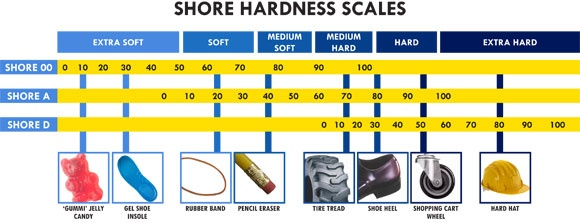
\includegraphics[width=\linewidth]{gfx/durometer}
	\caption[Shore hardness scales and everyday examples]{Shore types A, D, and OO in comparison with everyday examples of various hardnesses.\cite{smoothon-web}}\label{fig:shore}
	%http://www.smooth-on.com/images/durometer_with_logo_small_580.jpg
	%TODO use pdf instead of shitty jpg
\end{figure}

The silicone rubbers used for casting bracelet prototypes are both located on the Shore A scale. The softer Mold Star 15 Slow has a Shore A hardness of 15 that could be roughly compared to that of a rubber band according to figure \ref{fig:shore}, while the slightly harder Sorta-Clear 37 has a Shore A rating of 37, similar to that of a pencil eraser.%TODO cite datasheet

Both silicone products are two compound mixes that have to be added up and stirred before casting. While the Mold Star silicone has a rather low viscosity, casting the Sorta-Clear requires careful mold design, since it does not distribute well and is rather viscous. A vibrating table can help in filling the mold completely, but nonetheless were casts with the Sorta-Clear silicone much less fruitful, especially for the detailed molds of the one-piece designs (cf. section \ref{sec:silicone-prototypes}).

\section{Design Process and Prototype Manufacturing}

The design process for the interactive bracelet presented in this thesis went through different stages. At first, a 3D-printed casing was favored, but later on a cast silicone bracelet turned out to be more comfortable for the user. The different prototypes are explained in detail in the following sections.

\subsection{Rigid Designs}

The first approach that comes to mind when thinking about bracelet design is a cuff-like, rigid shape. From the CAD point of view, the first bracelet prototype consisted of a single rectangular profile rotated around a oval curve which was derived from a measured wrist. The bracelet's inside was hollow, that would be the storage space for all electronic components. The cuff's gap was just large enough for the wrist to fit through, although in reality, this lead to light scratches on the skin in combination with the rough texture of the printed material. In addition, the uniform thickness made this first prototype uncomfortable to wear, especially at the open ends. So this fist prototype had some clear downsides that were eliminated in the next iteration.

\begin{figure}[bth]
	\myfloatalign
	\subfloat[\ac{CAD} view]
	{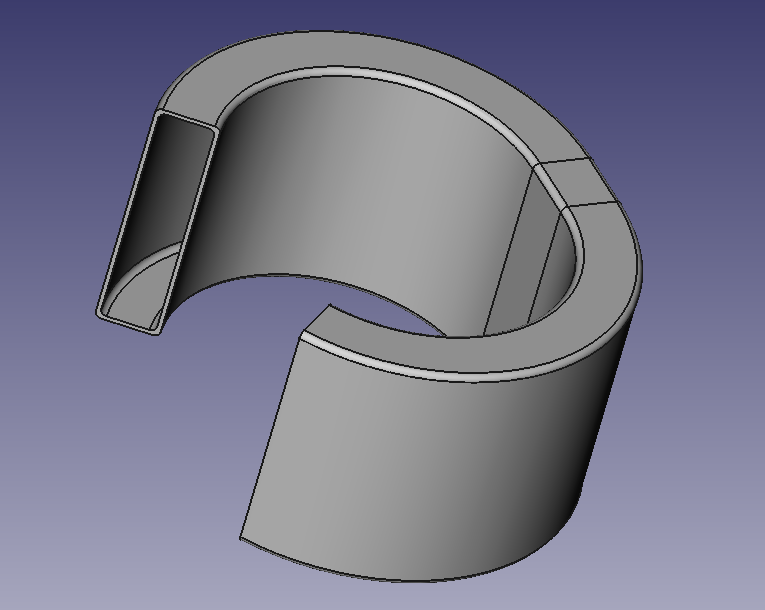
\includegraphics[width=.45\linewidth]{gfx/bracelet01-cad.png}} \quad
	\subfloat[Printed bracelet]
	{\label{fig:bracelet01}%
		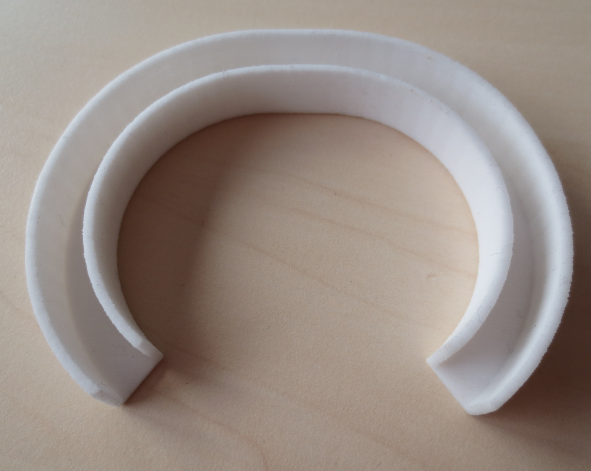
\includegraphics[width=.45\linewidth]{gfx/bracelet01-print-small.png}}
	\caption{First rigid design with uniform thickness}
\end{figure}

Due to a settings error in the PC that controls the 3D printer, the printout of this first design was aborted after one third of the process.

In the following iteration, a bracelet of varying thickness was designed to make wearing the prototype more comfortable. Decreasing the thickness from XX cm to YY cm made the look more appealing and wearing a little less clumsy. At the same time, the wall strength was decreased from X.Y mm to 0.7 mm, which made it very fragile in fabrication and usage, both prints broke during post-processing. Wearing the cuff while working on a PC feels only slightly uncomfortable, but twisting the hand is encumbered by the tight-fitting bracelet. A design goal for future prototypes derived from this prototype was adding more space between the arm and the bracelet to ensure better comfort while wearing it.

\begin{figure}[bth]
	\myfloatalign
	\subfloat[\ac{CAD} view]
	{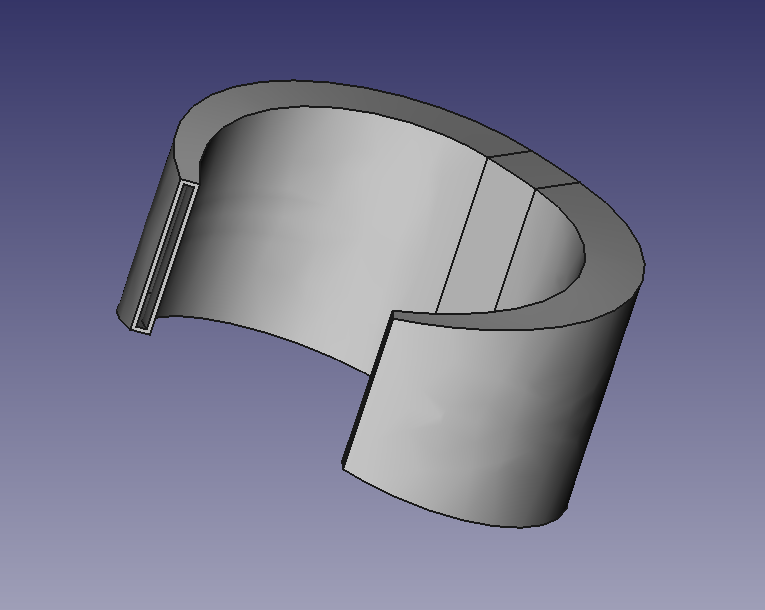
\includegraphics[width=.45\linewidth]{gfx/bracelet02-cad.png}} \quad
	\subfloat[Printed bracelet]
	{\label{fig:bracelet02}%
		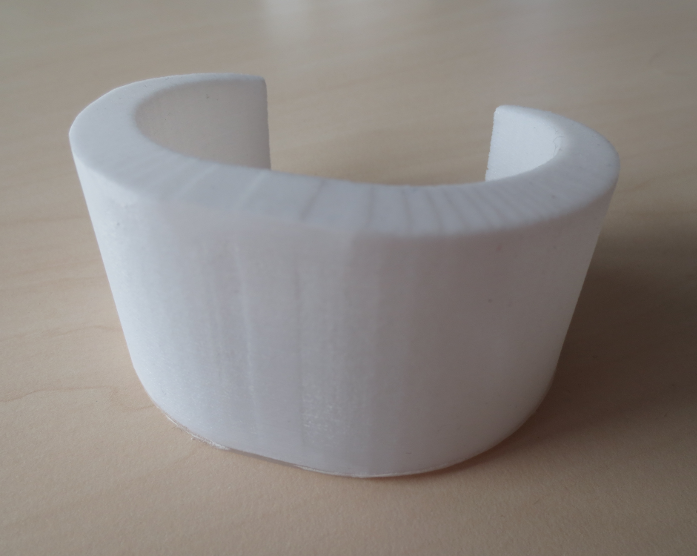
\includegraphics[width=.45\linewidth]{gfx/bracelet02-print-small.png}}
	\caption{Second design featuring a tapered shape}
\end{figure}

A modified design of the aforementioned prototype featured a removable lid since the tapered shape made it hard to access the inside space of the bracelet. The lid design was inspired by battery case covers commonly found in remote controls or small electronic devices. It features two nubsis on the one side that support the lid in its place and another, smaller nubsi with a cavity in the material right next to it, so the nubsi can snap just inside the lid gap when it closes.

\begin{figure}[bth]
	\myfloatalign
	\subfloat[Lid in \ac{CAD} view]
	{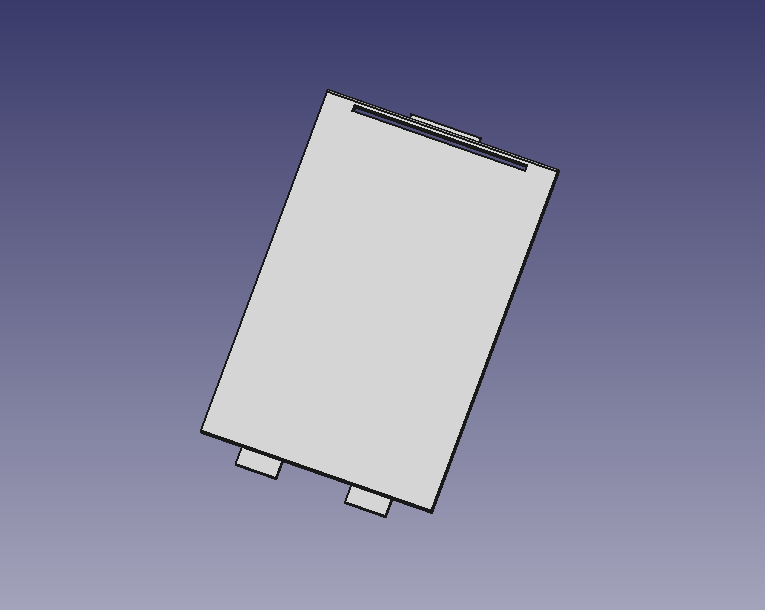
\includegraphics[width=.45\linewidth]{gfx/bracelet03-cad.png}} \quad
	\subfloat[Printed bracelet]
	{\label{fig:bracelet03}%
		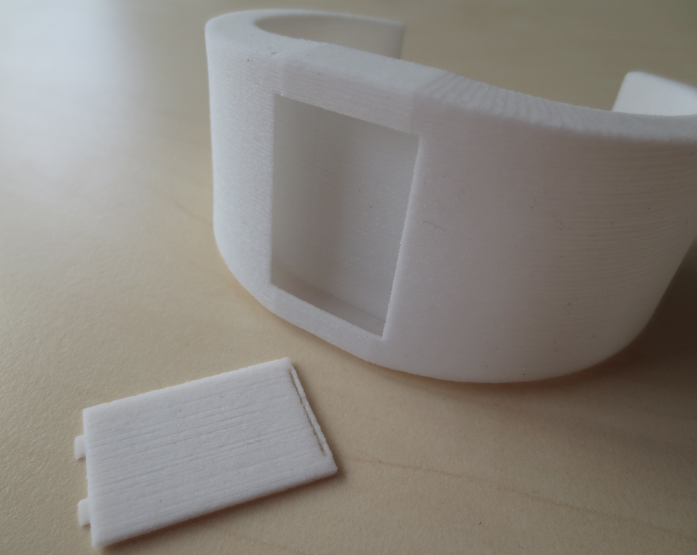
\includegraphics[width=.45\linewidth]{gfx/bracelet03-print-small.png}}
	\caption{Third design with removable lid}
\end{figure}

It turned out that the lid features were designed too fine, especially the flexible part was too thin to work as intended. The lid had to be opened and closed very cautiously and overall, the construction seemed not reliable for daily use. In addition, the rigid shape still lead to clumsiness in wearing the bracelet, so the whole concept of rigid bracelets was left behind.

\subsection{Segmented Designs}

The search for a more flexible printed bracelet shape lead to an entry for an activity bracelet design contest by Daniel Muschke on a 3D printing template exchange site called \textit{GrabCAD} \cite{amicobracelet}. Muschke created a \ac{CAD} file for a bracelet consisting of three segments that are connected by slow hinges. This design considered the electronic components like a micro-controller and a micro \ac{USB} port which made a good start for further modification, but unfortunately the file format made it impossible to alter the design in detail. A print was possible since \ac{STL} files were included in the upload. However, the design turned out to be too small to be actually wearable, but it demonstrated that printed hinges work well with a pivot made from wire. The style felt more comfortable to wear than the precious prototypes and felt leaner on the wrist than the rigid prototypes. Overall, the printed design looked promising so the idea of a tri-part bracelet was investigated further.

Recreating Muschke's design was not as easy as planned, since the parametric modeling approach was very different in comparison with previous designs. The first prototypes were based on a wrist-like circumference curve, while the multi-part design originated from a partitioned circle, since all parts should have the same dimensions in length and curvature. Adjusting the part size to the designated wrist turned out to be difficult, and prints of the design were either too small or too big.

The bracelet segments are hollow and open on the side that lays to the wrist, this leaves enough space for storing electronics. Since the parts are only connected by hinges, routing the necessary wires between the segments needs to be considered, e.g. by leaving small holes right next to the hinges.

\begin{figure}[bth]
	\myfloatalign
	\subfloat[\ac{CAD} view]
	{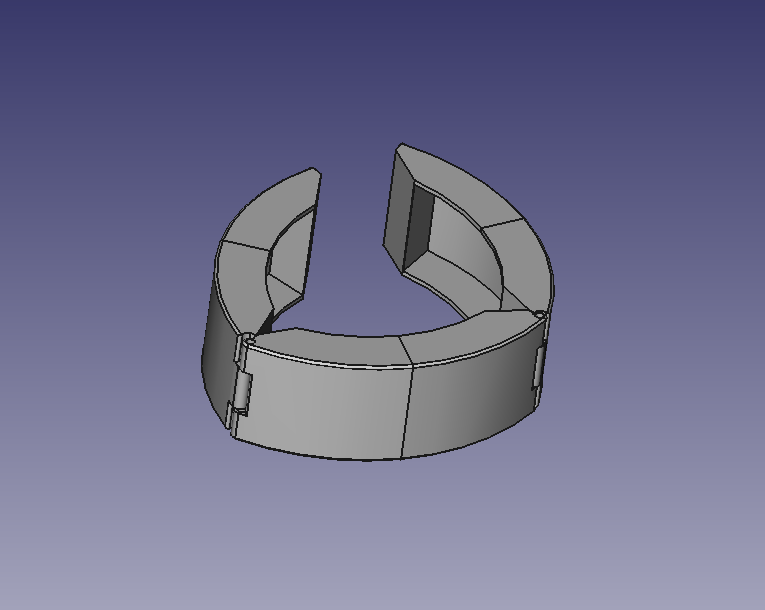
\includegraphics[width=.45\linewidth]{gfx/bracelet04-cad.png}} \quad
	\subfloat[Hinge Detail]
	{\label{fig:bracelet04}%
		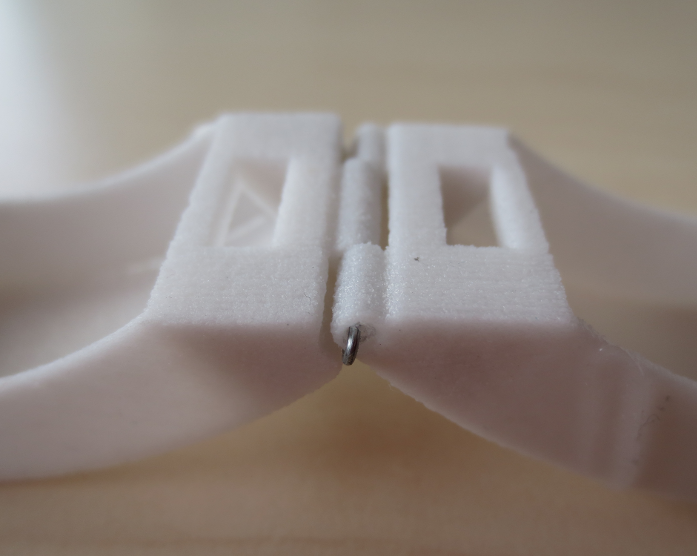
\includegraphics[width=.45\linewidth]{gfx/bracelet04-print-small.png}}
	\caption{Multi-part design}
\end{figure}

Since the manufacturing techniques offered at the \ac{HCI} group don't allow for slow hinges (as the inspiration by Muschke suggests), a different solution for keeping the bracelet closed while worn on the wrist needed to be considered. A magnet clasp with small neodymium magnets was tested, but attaching them turned out to be more difficult than expected. When attached to the inside of the segment tips, the magnetic force was too weak for reliably keeping the bracelet together. Mounting the magnets on the outside of the segments resulted in mounting difficulties, since the magnetic force of neodymium magnets is very strong and frequently resulted in torn glue layers.

When an electrophoretic display was considered to be part of the bracelet, the segmented approach became undesired, since in addition to aforementioned difficulties, the usable surface space was relatively small when it came to hosting a single big component like a display. This issue led to further research into various other manufacturing techniques and potential materials for bracelet prototypes, and eventually led to cast silicone.

\subsection{Silicone Bracelet}

After some consideration on a flexible e-ink display, a prototype bracelet made of silicone was considered. The molds used in the casting process were designed and printed just as the bracelets presented in the previous sections. However, designing a mold was significantly more difficult.

As with 3d printed prototypes, the bracelet positive was designed first. The flexibility of silicone allows for some features that weren't practical when implemented in rigid material, for example cavities for electronic components. This resulted in overall more complex bracelet concepts. In addition, closing mechanisms like magnets had to be considered in this design stage.

When the \ac{CAD} process for the positive is finished, the mold is successively designed by adding surrounding geometries to the model and applying boolean difference operations. If reuseability is desired for individual mold components or the whole mold, the geometry and constellation of the mold parts needs to be considered and the characteristics of the printed material have to be taken into consideration. For example... %TODO
Another important aspect of mold design is planning the casting process. Some types of silicone are more viscous than others, and the mold design needs to make sure that the liquid rubber reaches all corners and delicate parts well. The distribution inside the mold can be supported by applying gentle vibration during the cure process, but this assumes that the liquid silicone is already distributed into most regions of the mold.

The first silicone design was a simple strap with an open pocket for the long electrophoretic display and some cavities for a magnet clasp.

Mold design turned out a little tricky but finally succeeded. A two-piece mold was printed which only needed a little post-processing to fit properly together. The mold was coated with black spray paint to make the inside a little smoother, but this didn't work as intended so the painting step could be omitted in future mold making processes. The filling holes for the silicone were too small, and the mixture was more viscous than expected.

The first cast with a closed mold and filling through the holes was unsuccessful; it produced two small end pieces and nothing in between. For following casts, one part of the mold was filled with silicone and closed afterwards; this turned out significantly better. The orientation in which the mold is placed during the dry period is also relevant, as air bubbles will float towards the ``top'' of the mold, leading to instabilities when oriented inappropriately. Getting the silicone part out of the mold was no problem.

This first rubber bracelet design involved a magnet clasp, but it was infeasible to reliably attach magnets to silicone with anything but silicone itself and they would likely jump out of place and snap together if placed too close to each other in the design.

Two casts were made, one with each of the available silicone mixtures. The softer one was slightly too soft and had a disappealing color. In addition, the cavity rims were too short, so the display would jump out of place almost instantly when bending the bracelet.

\subsection{One-Piece Silicone Bracelet}
The next design was a ring-like silicone bracelet in one piece, so the issue with the clasp was no concern. The mold for this prototype consisted of three pieces, two rings and a bottom plate. Due to the very rigid characteristic of the printed material, the molds could not be recovered after the cast and had to be destroyed. In order to prevent unnecessary waste of material, the wall strength was reduced to 2.5 mm which turned out to be strong enough to survive the cast. The advantage of using one-time molds was the possibility to add tunnels to the design. This was used especially for the display area.

This mold was much harder to fill with silicone than the previous one. Especially the Sortaclear silicone was too viscous to fill the complete mold, resulting in broken casts. The green MoldStar silicone turned out to work quite well. A simple vibrating plate made with a servo monitor with some scrap materials as an imbalance glued onto a plastic tray helped filling all parts of the mold and reducing air bubbles in the cast. The design also features wider cavity rims to hold the display in place and first wearing tests resulted in success.

The design was iterated several times as the hardware components were layouted on a \ac{PCB} shield and the display was omitted for initial interaction tests.

\section{Teensy Development Board}
The core part of the bracelet's electronics is the Teensy USB development board, which is built around a MK20DX256
32 bit ARM Cortex-M4 Processor running on 72 MHz clock speed \cite{teensy_web}.

\section{Touch Slider}
The major input interface of the bracelet is a touch surface which consists of cut copper foil placed underneath the electrophorus display.
%TODO explain capacitive touch
%TODO explain geometry
%TODO explain interference sources

\section{3D Accelerometer}
%TODO how it works
%TODO I2C

\section{Flexible Electrophoretic Display}